\chapter{Related Work}\label{ch:related-work}

To answer the main thesis question, a review of existing studies will be needed.
The topic of DQ and the cost on business is well researched.
One of the oldest articles was written by Gerald A. Feltham in 1968 with title \enquote{The Value of Information}.
Many articles and studies were written on the topic since then, therefore we can recognize some basic structures when talking about DQ methodology.

\section{Hybrid Approach}

In the article \textit{Data quality assessment: The Hybrid Approach} the authors defined data quality as \enquote{fit for use}.
They reviewed several assessment techniques, including:
\begin{itemize}
    \item AIMQ (Lee et al., 2002),
    \item TQDM (English, 1999),
    \item cost-effect of low data quality (Loshin, 2004) and
    \item subjective-objective data quality assessment (McGilvray, 2008).
\end{itemize}

The result of the study is a general framework for creating customized, bussiness unique data quality assessment process.
The process consists of seven consecutive activities:
\begin{enumerate*}[label=(\roman*)]
    \item select data items,
    \item select a place where data is to be measured,
    \item identify reference data,
    \item identify DQ dimensions,
    \item identify DQ metrics,
    \item perform measurement and
    \item conduct analysis of the results.
\end{enumerate*}

The methodology can be summarized as follows.
The input data (i) are measured (vi) and thus the dimensions (iv) and metrics (v) are obtained.
Metrics are applied to the data in the central repository (ii).
If necessary, the data may be validated against the reference data (iii).

\begin{figure}[htb]
    \centering
    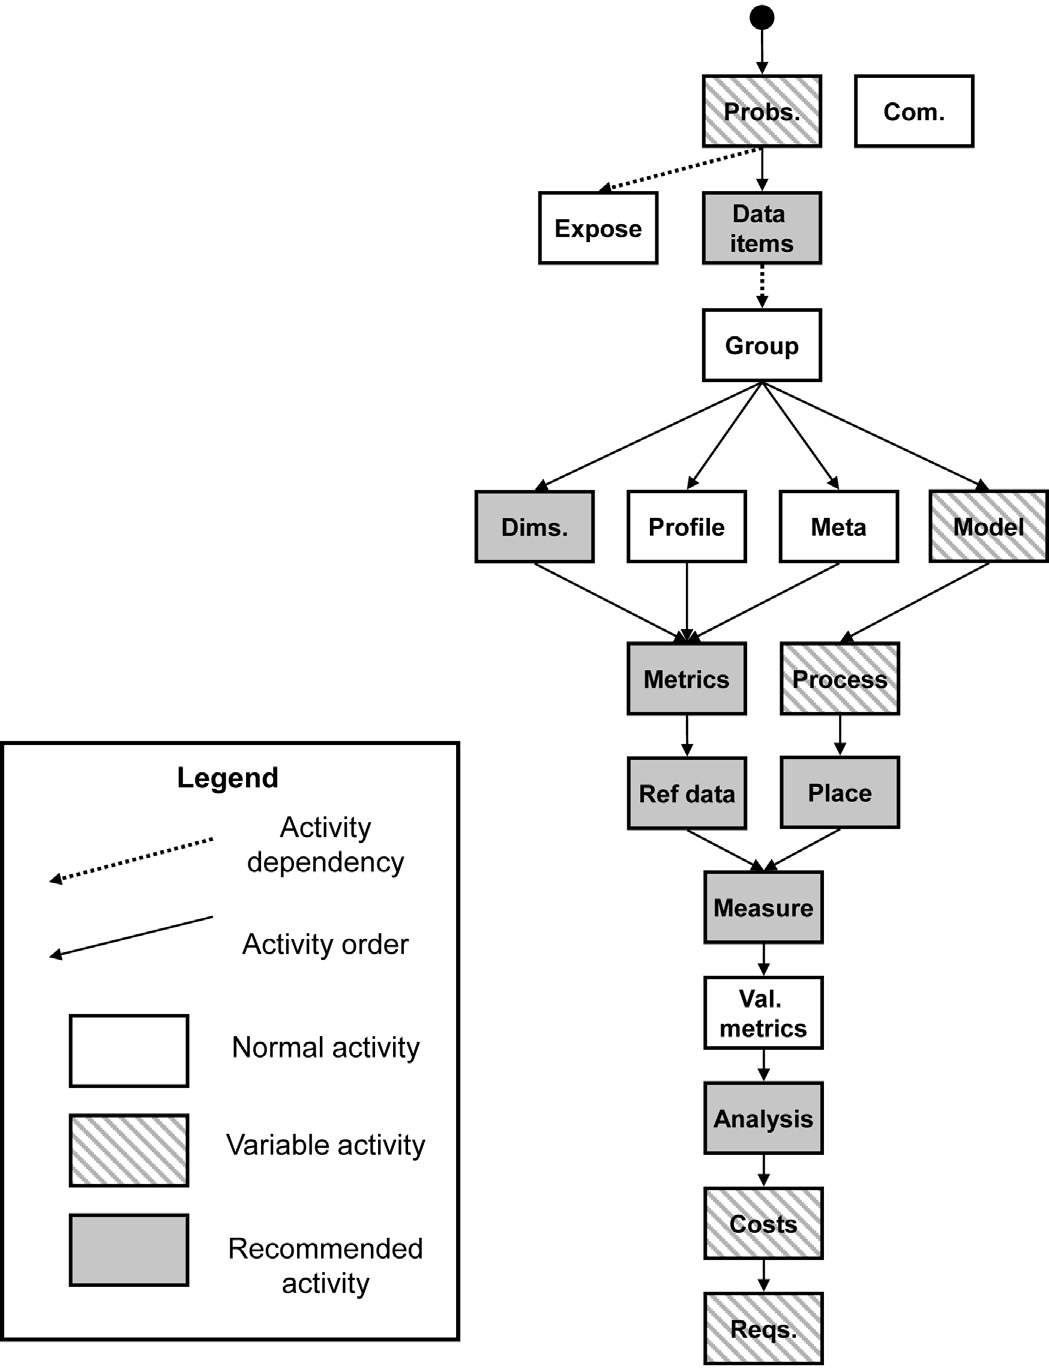
\includegraphics[width=0.4\textwidth]{figures/hybrid-generic-at.jpg}
    \caption{A generic AT according to the Hybrid Approach methodology~\cite{woodal2013}}
    \label{fig:hybrid-generic-at}
\end{figure}
\FloatBarrier

The methodology is tested by the authors on two practical cases.
The first use case is to adapt the framework for an MRO (Maintenance Repair and Operations) company.
The second use case is the adaptation of the methodology for the London Underground.

A very important result of the study is a configurable process model.
It is possible to design an alternative configuration of the process model to suit the case study or specific domain.

\begin{figure}[htb]
    \centering
    
    \begin{subfigure}{0.45\textwidth}
        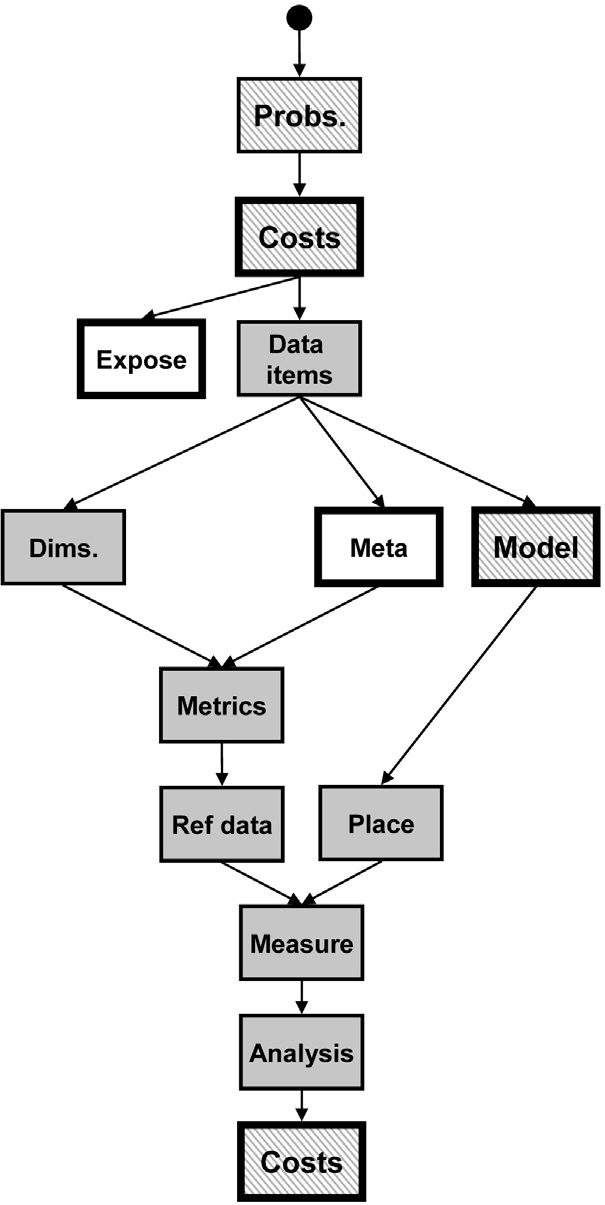
\includegraphics[height=7cm]{figures/hybrid-at-mro.jpg}
        \centering
        \caption{An AT for the MRO organisation}
        \label{fig:hybrid-at-mro}
    \end{subfigure}
    \begin{subfigure}{0.45\textwidth}
        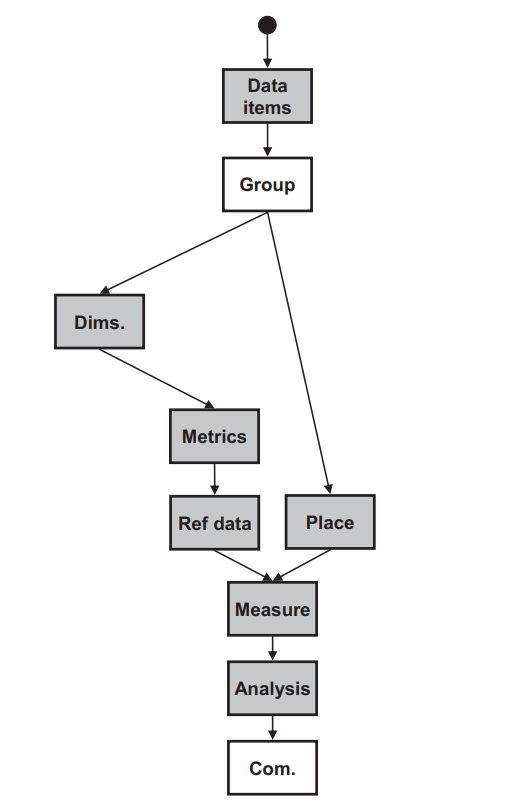
\includegraphics[height=7cm]{figures/hybrid-at-lu.png}
        \centering
        \caption{An AT for London Underground}
        \label{fig:hybrid-at-lu}
    \end{subfigure}

    \caption{ATs for the case studies~\cite{woodal2013}}
    \label{fig:bybrid-at}
\end{figure}
\FloatBarrier

In the \textit{Hybrid Approach}, the ATs developed between 1998 and 2008 were incorporated, and they all suggest very similar ideas to evaluating DQ~\cite{woodal2013}.
The methodology, thanks to the fact that it takes over the best practices of other methodologies, will be up-to-date for a long time.
The only problem arises when multiple stakeholders demand conflicting requirements.
If one party requires some activity and the other does not, the activity cannot simply be incorporated due to time and resource costs.
A thorough analysis is needed in this regard.

\section{AIM Quality}

The AIM Quality is a information quality assessment and benchmarking methodology for Management Information Systems (MIS).
The methodology consists of three main components, a model, a questionnaire to measure information quality, and analysis techniques for information quality interpretation.
The methodology has been built on the foundations of other academic studies as well as professional white-papers (e.g., Department of Defense, HSBC, and AT\&T), and has been validated on health organizations use cases.

The important components in AIMQ are the IQ dimensions, critical for the information consumers.
The authors grouped IQ dimensions into four categories, \textit{intrinsic} IQ (the information itself contains a certain level of quality), \textit{contextual} IQ (quality must be considered within the business context), \textit{representational} IQ (expressing whether the information is comprehensible in the information system) and \textit{accessibility} IQ (expressing whether the information is accessible in the information system, but at the same time securely stored).

The information quality model in AIMQ, Product Service Provider (PSP/IQ) model, has four quadrants relevant to the IQ improvement decision process.
The model is shown in the Table~\ref{table:psp-iq}.
This model can be used to evaluate how well a company develops \textit{sound} and \textit{useful} information products and delivers \textit{dependable} and \textit{usable} information services to the consumers.

\begin{table}[htbp]
    \centering

    \begin{tabular}{@{}l|ll@{}}
        \toprule
                        & \shortstack{Conforms to \\ specifications}    & \shortstack{Meets or exceeds consumer \\ expectations}    \\ \midrule
        Product Quality & Sound information                             & Useful information                                        \\
        Service Quality & Dependable information                        & Usable information                                        \\
        \bottomrule
    \end{tabular}

    \caption{The PSP/IQ model~\cite{lee2002}}
    \label{table:psp-iq}
\end{table}
\FloatBarrier

\subsection{Four PSP/IQ model quadrants}

The next four paragraphs contain examples of DQ dimensions contained in each of the quadrants.

\paragraph*{Sound Information Dimensions} Free-of-error, Concise representation, Completeness, Consistent representation.
\paragraph*{Useful Information Dimensions} Appropriate amount, Relevancy, Understandability, Iterpretability, Objectivity.
\paragraph*{Dependable Information Dimensions} Timeliness, Security.
\paragraph*{Usable Information Dimensions} Believability, Accessibility, Ease of operation, Reputation.

\section{Comprehensive Data Quality Methodology}

A comprehensive data quality methodology (CDQM) for web and structured data is a methodology developed by Batini et al. (2008).
The methodology consists of three main phases: 
\begin{enumerate*}[label=(\roman*)]
    \item state reconsruction (modeling of organizational context),
    \item assessment (problem identification and DQ measurement) and
    \item choice of the optimal improvement process.
\end{enumerate*}
From the last phase there is feedback to the previous phase.

\begin{figure}[htb]
    \centering
    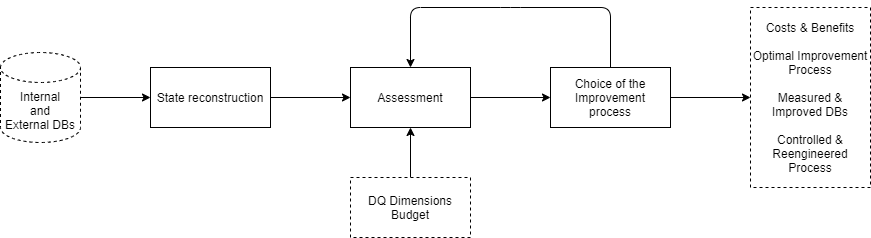
\includegraphics[width=0.9\textwidth]{figures/cdqm-diagram.png}
    \caption{Diagram of the CDQ methodology~\cite{batini2008}}
    \label{fig:cdqm-diagram}
\end{figure}
\FloatBarrier

\subsection{State reconstruction}

In the state reconstruction phase, the business/organizational context linked to internal and external data is modelled in terms of organizational units, processes, and rules~\cite{batini2008}.
This phase offers an overview of data providers and users, the flow of data and the use of data between them~\cite{batini2008}.

The state of data and their use-cases are recreated int he first step.
For a meaningful representation of this knowledge, two matrices are used.
The first one is Data Organizational Unit matrix.
The matrix's cells indicate whether an organizational unit generates (i.e., owns) or utilizes a collection of data.
The second one is Dataflow Organizational Unit matrix.
In this case, each cell of the matrix indicates whether an entity is a data flow consumer or provider~\cite{batini2008}.

In the second step, the Process Organizational Unit matrix identifies and describes the owner and contributing units for each process.
This matrix assists in the delegation of responsibility for quality improvement activities~\cite{batini2008}.

This step helps in provisioning of a comprehensive view of organizational processes and, as a result, aids in the decision-making process for quality improvement activities~\cite{batini2008}.
The Service Norm Process matrix is built to provide the information on how each macroprocess produce services for the clients and how the processes cooperate in the production of those services~\cite{batini2008}.

\subsection{Assessment}

In the assessment phase, internal and external users are involved to identify relevant DQ issues.
After obtaining information about the DQ issues, it is necessary to define quantitative metrics to evaluate the severity of DQ problems.

\begin{table}[htbp]
    \centering

    \begin{tabular}{@{}lllll@{}}
        \toprule
        Quality dimension/database  & \shortstack{Duplicate \\ objects} & \shortstack{Matching \\ objects}  & Accuracy  & Currency          \\ \midrule
        Social Security DB          & 5\%                               &                                   & 98\%      & 3 months delay    \\
        Accident Insurance DB       & 8\%                               &                                   & 95\%      & 5 months delay    \\
        Chamber of Commerce DB      & 1\%                               &                                   & 98\%      & 10 months delay   \\
        The three databases         &                                   & 98\%                              &           &                   \\
        \bottomrule
    \end{tabular}

    \caption{Example databases, quality dimensions and metrics~\cite{batini2008}}
    \label{table:ex-dat}
\end{table}
\FloatBarrier

\subsection{Choice of the optimal improvement process}

The organisation must set target quality values \( DQ_{ij}^* \), based on actual quality values \( DQ_{ij} \) linked with the \textit{i-th} dataset and the \textit{j-th} quality dimension, to be achieved through the improvement process~\cite{batini2008}.
DQ targets are defined by performing a \textit{process-oriented} and a \textit{cost-oriented} analysis~\cite{batini2008}.

In the \textit{cost-oriented} analysis, the economic costs – that the business can afford for the DQ improvement process – needs to be defined.
A major obstacle is the difficulty of estimating costs and benefits in advance.

A \textit{non-quality costs} (\( C_{ij} \)) are the costs associated with poor data quality and, therefore, with all the inevitable activities to correct errors and re-execute tasks~\cite{batini2008}.
The evaluation of quality targets is in the Figure~\ref{fig:cdqm-q}.

\begin{figure}[htb]
    \centering
    
    \begin{subfigure}{0.45\textwidth}
        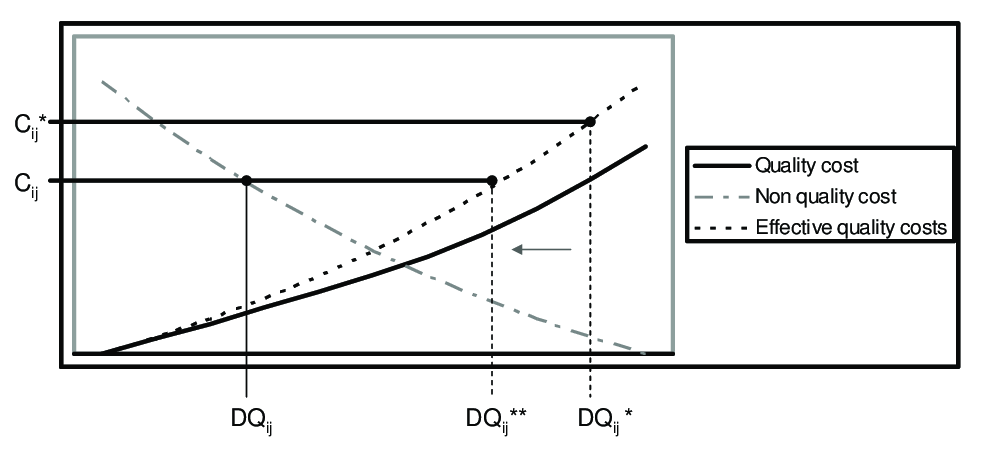
\includegraphics[width=\textwidth]{figures/cdqm-less-q.png}
        \centering
        \caption{Evaluation of less ambitious quality targets}
        \label{fig:cdqm-less-q}
    \end{subfigure}
    \begin{subfigure}{0.45\textwidth}
        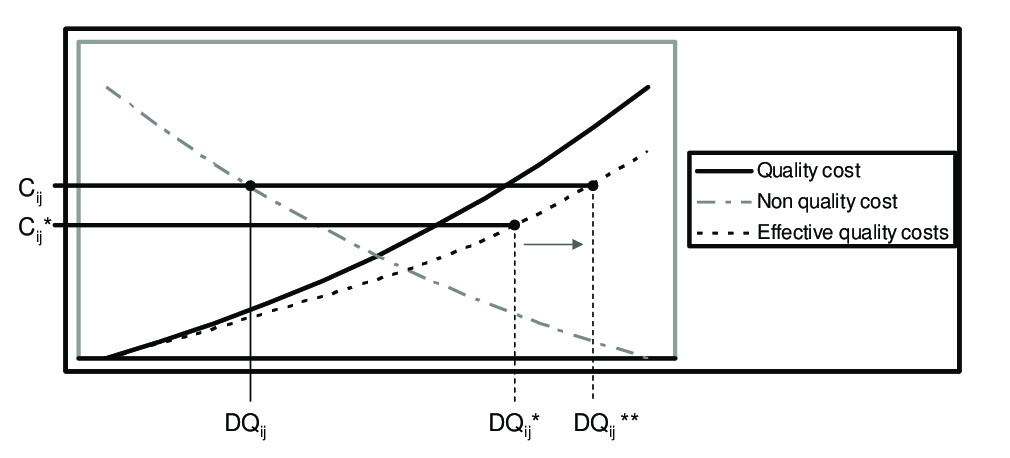
\includegraphics[width=\textwidth]{figures/cdqm-more-q.png}
        \centering
        \caption{Evaluation of less ambitious quality targets}
        \label{fig:cdqm-more-q}
    \end{subfigure}

    \caption{Evaluation of quality targets~\cite{batini2008}}
    \label{fig:cdqm-q}
\end{figure}
\FloatBarrier

\section{Business Oriented Data Quality}

Otto et al. (2011) developed a design process for the identification of business oriented DQ metrics~\cite{otto2011}.
The paper does not present any concrete DQ metrics even though they studied data quality problems in three companies.
Instead, those three companies' data problems were used to create an assumption that data defects cause business problems~\cite{otto2011}.
According to Otto et al. (2011), the identification of DQ metrics therefore should be based on how the data impacts process metrics~\cite{otto2011}.

A method engineering (ME) is used to design the framework.
Methodology therefore consists of five components:
\begin{enumerate*}[label=(\roman*)]
    \item design activities,
    \item design results,
    \item meta-model,
    \item roles and
    \item techniques.
\end{enumerate*}

\subsection{Meta-model}

Otto et al. (2011) describe entities and relations used to characterize the activities of the procedure model~\cite{otto2011}.

\begin{figure}[htb]
    \centering
    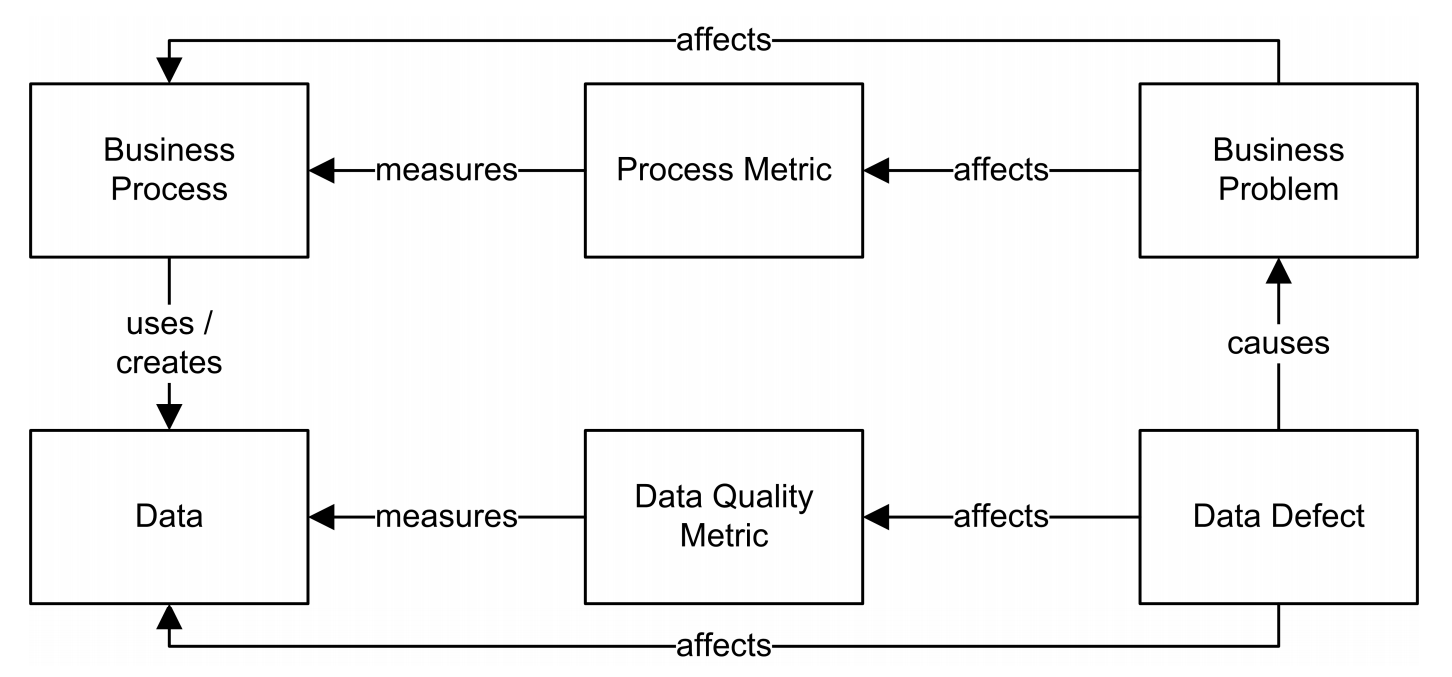
\includegraphics[width=0.9\textwidth]{figures/otto-figure-1.png}
    \caption{Entities and relations of a business oriented data quality metric~\cite{otto2011}}
    \label{fig:otto-figure-1}
\end{figure}
\FloatBarrier

\subsubsection{Business Problem}

Business problem is either system state (e.g. the package cannot be delivered) or incident (e.g. scrap parts production) causing decrease of system performance, therefore impacts \textit{process metrics} results.
It directly impacts business process and is defined by \textit{probability of occurence}\footnotemark and \textit{intensity of impact}\footnotemark.

\footnotetext[1]{Probability of occurence of event \( E \) can be denoted as \( P(E) = \frac{r}{n} \), where \( r \) is number of ways \( E \) can happen from all possible ways \( n \), \( P(E) \in [0, 1] \).}
\footnotetext[2]{
    Intensity of impact is a measure of the time-averaged power density of a wave at a particular location.
    In our case, intesity should be defined as \( I = \frac{\langle BC \rangle}{BA} \), where \( \langle BC \rangle \) is time-averaged business cost of problem and \( BA \) business area through which the problem propagates during certain time frame, \( I \in [0, \inf] \).
    If we define business area as sum of employees impacted by problem and their time spend to solve it, the unit of intensity would be costs per hour.
}

\subsubsection{Business Process}

By business process is meant sequence of tasks intended to generate value for customer and profit for the company.
The business process is controlled and defined as part of a~business strategy with corresponding modeling and measuring tools such as BPMN~2.0 or Key Performance Indicators (KPIs).

\subsubsection{Process Metric}

Quantitative measure of the degree to which a process fulfill a given quality attribute (e.g. scrap rate).

\subsubsection{Data}

Data is representation of objects and object relations.

\subsubsection{Data Defect}

It is an incident (e.g. wrong entered data), causing value decrease of data quality metrics.
As well as \textit{business problem}, a data defect poses a risk in terms of \textit{probability of occurence} and \textit{intensity of impact}.

\subsubsection{Data Quality Metric}

Quantitative measure of the degree to which data fulfill a given quality attribute (e.g. accuracy, consistency, currency,\ldots).

\subsection{Procedure Model}\label{subsec:procedure-model}

Procedure model defined by Otto et al. (2011) consists of three phases and seven activities.
Activity flow model is shown in the figure~\ref{fig:otto-figure-2}.
Letter color codes under the activities indicate degree of usage in the respective companies mentioned in the paper.
Black color means that activity was fully used, grey color means partial usage and white indicates no use at all.

\begin{figure}[htb]
    \centering
    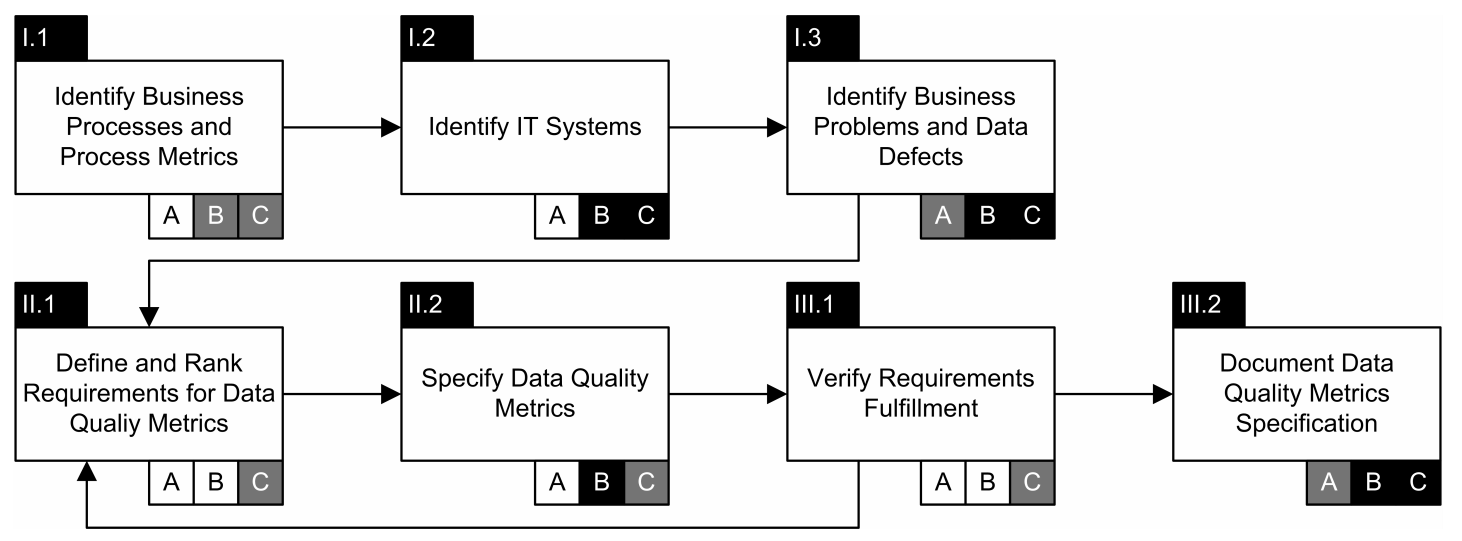
\includegraphics[width=0.9\textwidth]{figures/otto-figure-2.png}
    \caption{Procedure model and degree of usage of activities in each case~\cite{otto2011}}
    \label{fig:otto-figure-2}
\end{figure}
\FloatBarrier

\subsubsection{Phase 1}

First phase is used to collect information.
It consists of three activities:

\begin{enumerate}
    \item Identify Business Processes and Process Metrics,
    \item Identify IT Systems,
    \item Identify Business Problems and Data Defects.
\end{enumerate}

\subsubsection{Phase 2}

Second phase is used to specify requirements and design data quality mestrics.
It consists of two activities:

\begin{enumerate}
    \item Define and Rank Requirements for Data Quality Metrics,
    \item Specify Data Quality Metrics.
\end{enumerate}

\subsubsection{Phase 3}

Third phase is intended to approve and decument results.
As well assecond phase, this one consists of two activities:

\begin{enumerate}
    \item Verify Requirements Fulfillment,
    \item Document Data Quality Metrics Specification.
\end{enumerate}

\subsection{Roles}

In the last part, the authors declare six roles and their assignment to activities from section~\ref{subsec:procedure-model}.
Those roles are:
\begin{enumerate*}[label=(\roman*)]
    \item Chief Data Steward,
    \item Business Data Steward,
    \item Technical Data Steward,
    \item Process Owner,
    \item Process user and
    \item Sponsor.
\end{enumerate*}

\section{ORME}

Batini et al. (2007) provided DQ assessment methodology called ORME (from italian word \enquote{orme} meaning track or trace).
The methodology consists of four Data Quality Risk evaluation phases:
\begin{enumerate}
    \item prioritization,
    \item identification,
    \item measurement,
    \item monitoring~\cite{batini2007}.
\end{enumerate}

The authors provided a comprehensive classification of the costs of poor data quality in their work.
In short, they classified costs into three categories:
\begin{itemize}
    \item current cost of insufficient data quality,
    \item cost of IT/DQ initiative to improve current quality status,
    \item benefits gained from improvement initiative implementation~\cite{batini2007}.
\end{itemize}

\subsection{Prioritization}

In this phase the model reconstruction happen.
All the relationships among organization units, processes, services and data are put together and organized e.g. in the form of matrices (database/organization matrix, dataflow/organization matrix, database/process matrix)~\cite{batini2007}.
The main goal is to provide map of the main data use across data providers, consumers and flows~\cite{batini2007}.

\subsection{Identification}

This phase main focus is on identification of loss events and definition of overall economic loss metrics~\cite{batini2007}.
In this case, loss can be expressed in 
\begin{enumerate*}[label=(\roman*)]
    \item absolute values (e.g. 100 USD),
    \item a~percentage with respect to reference variables (e.g. 10\% of GDP), or
    \item a~qualitative evaluation (e.g. low-medium-high)~\cite{batini2007}.
\end{enumerate*}

\subsection{Measurement}

In this phase actual qualitative and quantitative assessment of data quality is conducted.

\subsection{Monitoring}

The last phase establishes a feedback loop and threshold in the DQ assessment process.
DQ dimensions should be, according to the authors, evaluated periodically.
Therefore quality rule violation allerts and automatic processes should be defined in order to ensure required DQ levels~\cite{batini2007}.

Authors suggest discriminant analysis as an easy and effective way of loss event identification.
The goal is to identify loss event based on set of new values in the data source.
The model is build on a training set, with two classes (\textit{loss} and \textit{no loss}) in consideration.
A set of linear functions from predictors is constructed,

\begin{equation*}
    L = b_1 x_1 + b_2 x_2 + \ldots + b_3 x_3 + c
\end{equation*}

where \( b_k \) are discriminant coeficient, \( x_k \) are input variables (predictors) and \( c \) is a~constant~\cite{batini2007}.

\section{Data Quality and Security}\label{sec:data-quality-and-security}

Given the continuous risk of data braches, we should consider the impact of security mechanisms on data quality.
This topic is very timely, especially with the need to comply with the GDRP regulations.
Data Quality and Data Security are two key issues that address various problems in Data Engineering, such as large volumes and diversity of data, credibility of data and their sources, data collection and processing speed, and so on~\cite{talha2019}.
Confidentiality, Integrity, and Availability are the three key security assets defined in terms of data security~\cite{talha2019}.
The ISO/IEC 25010 standard defines each of these properties in detail~\cite{iso25010}.
Whereas in terms of data quality, there is no consensus on any of the properties that define data quality or the precise definition of each property~\cite{batini2009}.

The main point of data security principle, particularly confidentiality and integrity, is to protect data from unauthorized access.
However, implementing a comprehensive data quality management system necessarily requires unrestricted read and write access to all data~\cite{talha2019}.
Since the data quality system can share data with other systems or be accessed by individuals with different business interests, this requirement can lead to plenty of security issues~\cite{talha2019}.
As a result, data privacy can be a major obstacle to data quality.
Security exceptions may be required by a quality management system, which poses potential security risks.
This tensions between the two systems complicates their development and necessitates the emergence of new access control policies that allow quality processes to access the data they need without jeopardizing their security~\cite{talha2019}.
As Talha (2019) mentions, a sturdy \textit{access control model} such as TBAC (Task Based Access Control), RBAC (Role Based Access Control), ABAC (Attribute Based Access Control), OrBAC (Organization Based Access Control), PuRBAC (Purpose-Aware Role-Based Access Control) must be used to fulfill the policy.

\begin{figure}[htb]
    \centering
    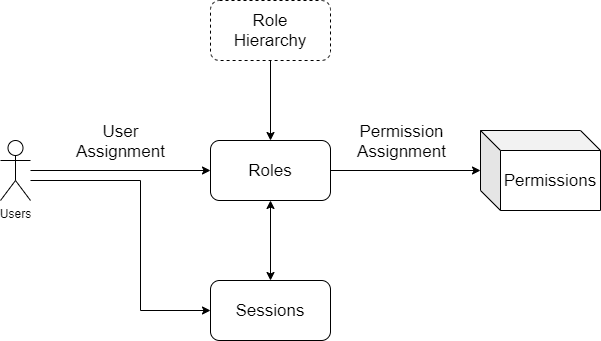
\includegraphics[width=0.7\textwidth]{figures/rbacm.png}
    \caption{Role Based Access Control Model}
    \label{fig:rbacm}
\end{figure}
\FloatBarrier

\textit{Differential privacy} has risen to prominence in applied mathematics as a leading data security technique, allowing accurate data analysis while preserving formal privacy guarantees~\cite{cummings2018}.
Data often contains \textit{sensitive attributes}, users' personal information, in a form of \textit{personal identifiers} or \textit{quasi-identifiers}.
\textit{Personal Identifiers} (PID) are data elements that identify a unique user in the dataset and allow another person to make the assumption of person's identity without their knowledge or consent (e.g., ID Number, Bank Account Number,\ldots).
A \textit{quasi-identifier} is a set of attributes that, when combined with external information, can be used to reidentify (or reduce uncertainty about) all or some of the entities to whom information is being referred (e.g., gender, postal code, age or nationality)~\cite{qid-springer}.

The personal data can be obscured using \textit{anonymization} techniques, allowing for accurate data analysis.
Narayanan (2008) proved, that \textit{anonymized} data can be \enquote{easily} recovered using \textit{linkage attack} (combining pieces of anonimized data to reveal one's identity).
To prevent data misuse (re-identification of users) after a security breach, several more advanced models – \textit{optimal k-anonymity}, \textit{l-diversity}, \textit{t-closeness} and \textit{differential privacy} – exists to safeguard individuals' personal information in datasets.

\begin{figure}[htb]
    \centering
    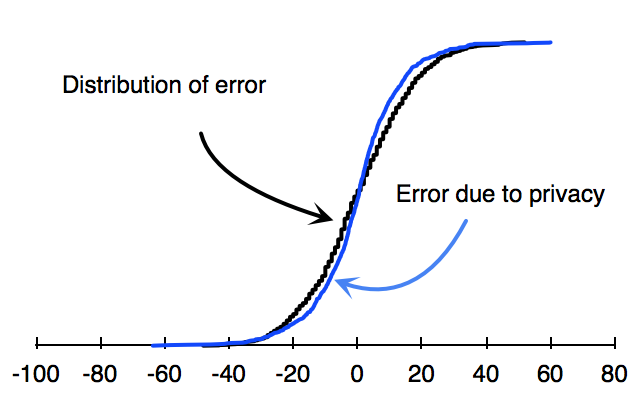
\includegraphics[width=0.7\textwidth]{figures/cdf3.png}
    \caption{Simplified explanation of differential privacy error~\cite{difpriv2016}}
    \label{fig:cdf3}
\end{figure}
\FloatBarrier

\textit{Differential privacy} algorithm stores complete and trusted data in some cases only.
In a certain subset of data, statistical noise is added, which compromises individual records (the record may or may not be true), but still allows accurate statistical analysis over the entire dataset~\cite{difpriv2016}.
By leveraging of Laplace distribution to spread data over a~large \textit{state space} and to increase the level of anonymity, the differential privacy model ensures that even if someone has full information on 99 of 100 people in a data collection, they will not be able to deduce information about the final user~\cite{web:differential-privacy,dwork2014}.
This mechanism is interesting because it certainly affects the quality of the data, but in a~different way than we would expect – making impossible to look at a specific record, but allowing analysis of the whole and the trend.

\section{Business Problems and Data Defects}

% Není možné mluvit o kvalitě dat a metodikách pro její zajištění, bez zmínky o konkrétních typech problémů, které se v rámci tématu vyskytují.
It is impossible to discuss data quality and methodologies for ensuring it without mentioning the specific types of issues that arise within the topic.
In the field of data engineering and data science, there are a number of common data defects.

\subsection*{Missing Data}

This is data that does not reach the destination data store~\cite{web:common-defects}.
This problem usually occurs when handling the data needed to clean up in the source database; by operating with invalid or incorrect lookup table in the transformation logic; or by invalid table joins.
An example of missing data is shown in Figure~\ref{fig:missing-data}.

\paragraph*{Example} We transform data from Task Management Solution.
Lookup table should contain a field value of \enquote{Minor} which maps to \enquote{Low}.
However, source data field contains \enquote{Mino} - missing the \textit{r} and fails the lookup, resulting in the target data field containing null.
If this occurs on a key field, a possible join would be missed and the entire row could fall out.

\begin{figure}[htb]
    \centering
    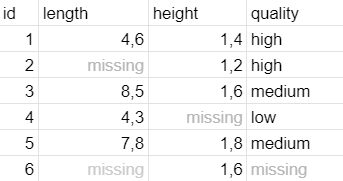
\includegraphics[width=.5\textwidth]{figures/missing-data.png}
    \caption{Missing Data}
    \label{fig:missing-data}
\end{figure}
\FloatBarrier

\subsection*{Truncation of Data}

Many data is being lost by truncation of the data fields.
This happens when there are invalid field lengths on target database or by transformation logic not taking into account field lengths from the source~\cite{web:common-defects}.

\paragraph*{Example} We transform financial data with complete exchange-traded fund (ETF) names.
Source field value \enquote{iShares Global High Yield Corp Bond UCITS ETF} is being truncated to \textit{varchar(32)}.
since the source data field did not have the correct length to capture the entire field, only \enquote{iShares Global High Yield Corp B} is stored.

% \begin{figure}[htb]
%     \centering
%     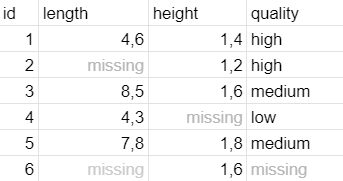
\includegraphics[width=.5\textwidth]{figures/truncation-data.png}
%     \caption{Data Truncation}
%     \label{fig:truncation-data}
% \end{figure}
% \FloatBarrier

\subsection*{Data Type Mismatch}

Data types not setup correctly on target database cause serious problems.
This usually happens when using ETL pipeline with an automatic or semi-automatic column type recognition~\cite{web:common-defects}.
% Data inženýr spoléhá na bezchybné rozpoznání datového typu a nezkontroluje správnost výstupních tabulek.
The data engineer relies on error-free data type recognition and does not check the accuracy of the output tables.

\paragraph*{Example} Source data field was required to be a \textit{varchar}, however, when initially configured, was setup as a \textit{date}.

% \begin{figure}[htb]
%     \centering
%     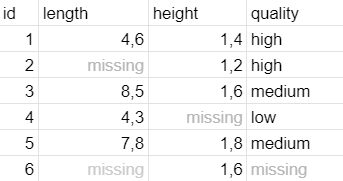
\includegraphics[width=.5\textwidth]{figures/mismatch-data.png}
%     \caption{Data Type Mismatch}
%     \label{fig:mismatch-data}
% \end{figure}
% \FloatBarrier

\subsection*{Null Translation}

In the source dataset, \textit{null} values are not being transformed to correct target values~\cite{web:common-defects}.
Development team did not include the \textit{null} translation in the ETL process.

\paragraph*{Example} A \enquote{Null} source data field was supposed to be transformed to \enquote{None} in the target data field.
However, the logic was not implemented, resulting in the target data field containing \enquote{null} values\footnotemark.

\footnotetext{
    None is a concept that describes the absence of anything at all (nothingness), while Null means \textit{unknown} (we do not know if there is a value or not).
}

% \begin{figure}[htb]
%     \centering
%     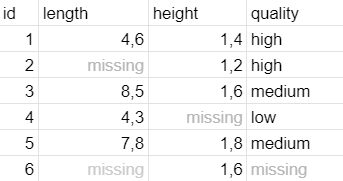
\includegraphics[width=.5\textwidth]{figures/null-translation.png}
%     \caption{Null Translation}
%     \label{fig:null-translation}
% \end{figure}
% \FloatBarrier

\subsection*{Wrong Translation}

Wrong translations happen when a source data field for \textit{null} was supposed to be transformed to \enquote{None} in the target data field, but was not transformed correctly~\cite{web:common-defects}.
The logic was not implemented, resulting in the target data field containing \textit{null} values.
Wrong translation is the exact opposite to \textit{Null Translation}.

\paragraph*{Example} Target field should only be populated when the source field contains certain values, otherwise should be set to null.
Let's look at a very basic example.
During analytical processing of medical data (e.g., list of patients with oncological finding), we need to set target field to \textit{true} if the one or multiple source values indicate certain treatment.
However, the target field is populated (either with blank charater or other values) although source values do not correspond to the required logic.

% \begin{figure}[htb]
%     \centering
%     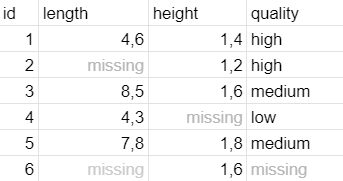
\includegraphics[width=.5\textwidth]{figures/wrong-translation.png}
%     \caption{Wrong Translation}
%     \label{fig:wrong-translation}
% \end{figure}
% \FloatBarrier

\subsection*{Misplaced Data}

If the source data fields are not being transformed to the correct target data fields, we call the issue \enquote{Misplaced Data}~\cite{web:common-defects}.
One of the possible causes is that development team inadvertently mapped the source data field to the wrong target data field.

\paragraph*{Example} A source data field was supposed to be transformed to target data field \enquote{Last\_Update}.
However, the development team inadvertently mapped the source data field to \enquote{Date\_Created}.

% \begin{figure}[htb]
%     \centering
%     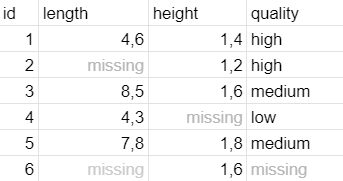
\includegraphics[width=.5\textwidth]{figures/misplaced-data.png}
%     \caption{Misplaced Data}
%     \label{fig:misplaced-data}
% \end{figure}
% \FloatBarrier

\subsection*{Extra Records}

Records which should be excluded in the ETL are included in the ETL.
This happens when developers do not include filter in their code~\cite{web:common-defects}.

\paragraph*{Example} If a record has the deleted field populated, the record and any data related to that record should not be in any ETL.

% \begin{figure}[htb]
%     \centering
%     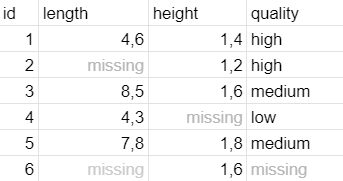
\includegraphics[width=.5\textwidth]{figures/extra-records.png}
%     \caption{Extra Records}
%     \label{fig:extra-records}
% \end{figure}
% \FloatBarrier

\subsection*{Not Enough Records}

Records which should be in the ETL are not included in the ETL.
Development team had a filter in their code which should not have been there~\cite{web:common-defects}.

\paragraph*{Example} If a record was in a certain state, it should be sent through ETL pipeline over to the data warehouse.

% \begin{figure}[htb]
%     \centering
%     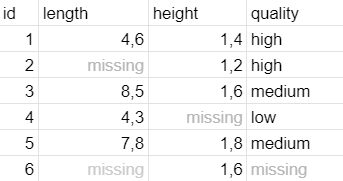
\includegraphics[width=.5\textwidth]{figures/notenough-records.png}
%     \caption{Not Enough Records}
%     \label{fig:notenough-records}
% \end{figure}
% \FloatBarrier

\subsection*{Transformation Logic Errors}

Testing sometimes can lead to finding \enquote{holes} in the transformation logic or realizing the logic is unclear~\cite{web:common-defects}.

Sometimes the processes are overly complicated, and the development team fails to account for special cases.
Most cases fall into a certain branch of logic for a transformation, but a small subset of cases (sometimes with unusual data) may not fall into any branches~\cite{web:common-defects}.
How the analytics and developers handles these cases could be different (and may both end up being wrong) and the logic is changed to accommodate the cases.
The next reason why this happens is that analytic and developer have different interpretation of transformation logic, which results in different values~\cite{web:common-defects}.
As a result, the logic is rewritten to make it more clear.

\paragraph*{Example} Foreign country cities that contain special language specific characters might need to be dealt with in the ETL code (e.g., Århus).

% \begin{figure}[htb]
%     \centering
%     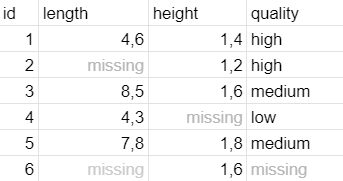
\includegraphics[width=.5\textwidth]{figures/logic-errors.png}
%     \caption{Transformation Logic Errors}
%     \label{fig:logic-errors}
% \end{figure}
% \FloatBarrier

\subsection*{Simple and Small Errors}

Capitalization, spacing and other small errors cause problems with data.
Data inconsistencies are easy to fix, but happen often~\cite{web:common-defects}.
The only real solution is to always double check data and ETL procedure~\cite{web:common-defects}.

% \begin{figure}[htb]
%     \centering
%     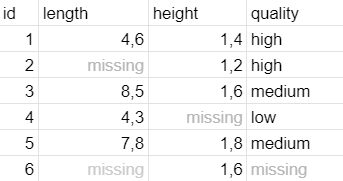
\includegraphics[width=.5\textwidth]{figures/small-errors.png}
%     \caption{Simple and Small Errors}
%     \label{fig:small-errors}
% \end{figure}
% \FloatBarrier

\subsection*{Sequence Generator}

Ensuring that the sequence number of reports are in the correct order is very important when processing follow up reports or answering to an audit.
If the sequence generator is not configured correctly, procedure results in records with a duplicate sequence number~\cite{web:common-defects}.

\paragraph*{Example} Duplicate records in the sales report were doubling up several sales transactions which skewed the report significantly.

% \begin{figure}[htb]
%     \centering
%     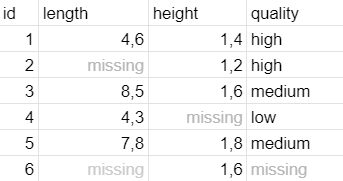
\includegraphics[width=.5\textwidth]{figures/sequence-generator-error.png}
%     \caption{Sequence Generator Error}
%     \label{fig:sequence-generator-error}
% \end{figure}
% \FloatBarrier

\subsection*{Undocumented Requirements}

During ETL development, sometimes certain requirements are found, that are \enquote{understood} but are not actually documented anywhere.
This causes issues when members of the development team do not understand or misunderstood the undocumented requirements~\cite{web:common-defects}.

\paragraph*{Example} ETL pipeline contains a restriction in the \enquote{where} clause, limiting how certain reports are brought over.
Moreover, there were used mappings that were understood to be necessary, but were not actually in the requirements.
Occasionally, it turns out that the understood requirements are not what the business wanted.

\subsection*{Duplicate Records}

Duplicate records are two or more records that contain the same data.
This issue happens when development team does not add the appropriate code to filter out duplicate records or there is some unexpected error in data generators.

\paragraph*{Example} Duplicate records in the sales report were doubling up several sales transactions which skewed the report significantly.

% \begin{figure}[htb]
%     \centering
%     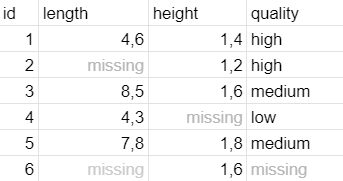
\includegraphics[width=.5\textwidth]{figures/duplicate-records.png}
%     \caption{Duplicate Records}
%     \label{fig:duplicate-records}
% \end{figure}
% \FloatBarrier

\subsection*{Numeric Field Precision}

Numbers that are not formatted to the correct decimal point or not rounded per specifications cause precision problems.
This has several causes, development team rounded the numbers to the wrong decimal point, used wrong rounding type or used wrong data type which lead to faulty rounding~\cite{web:common-defects}.

\paragraph*{Example} The sales data did not contain the correct precision and all sales were being rounded to the whole dollar.

\subsection*{Rejected Rows}

Data rows that get rejected by ETL process due to data issues.
Development team did not take into account data conditions that break the ETL for a particular row~\cite{web:common-defects}.
An example of an ETL process with rejected rows is shown in Figure~\ref{fig:rejected-rows}.

\paragraph*{Example} Missing data rows on the sales table caused major issues with the end of year sales report.

\begin{figure}[htb]
    \centering
    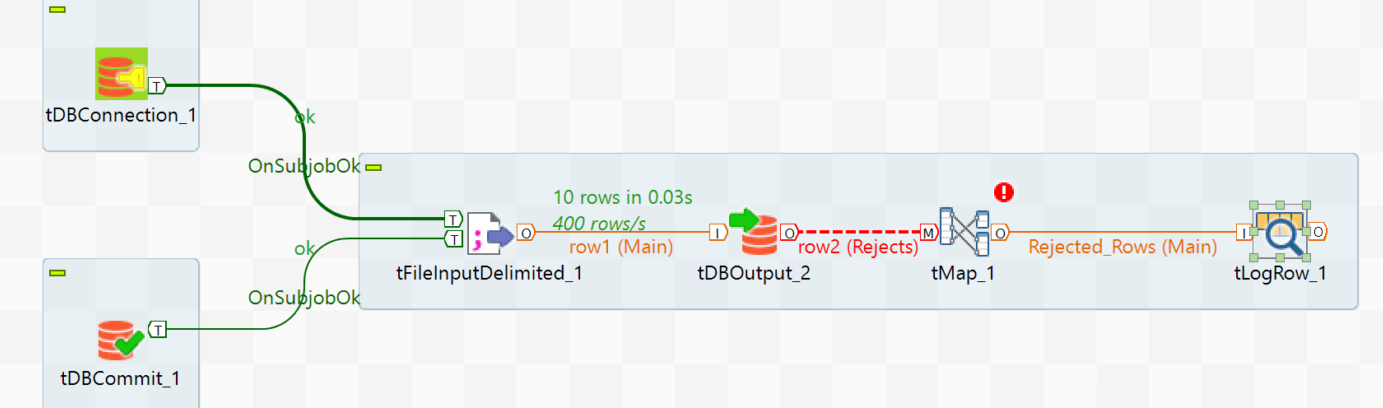
\includegraphics[width=.8\textwidth]{figures/rejected-rows.png}
    \caption{Talend ETL Rejects Rows}
    \label{fig:rejected-rows}
\end{figure}
\FloatBarrier

% Two main perspectives on Data Quality Management:
% Broad Perspective (from the enterprise poin of view on the lifecycle of data circulating in the company)~\cite{book:dama}
% Narrow Perspective (from the viewpoint of tasks to be done by data management professionals)~\cite{pres:dcam}

% \section{Requirements for Data Quality Metrics}

% TODO

% \subsection{Existence of minimum and maximum metric values}

% TODO

% \subsection{Interval-scaled metric values}

% TODO

% \subsection{Quality of the configuration parameters and the determination of the metric values}

% TODO

% \subsection{Sound aggregation of the metric values}

% TODO

% \subsection{Economic efficiency of the metric}

% TODO

% \section{Other}

% \begin{figure}[htb]
%     \centering
%     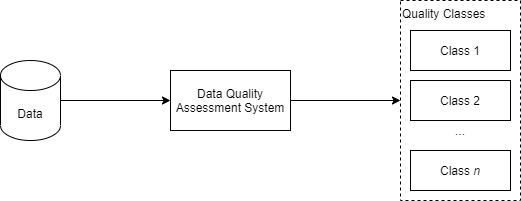
\includegraphics[width=0.9\textwidth]{figures/dq-simple.png}
%     \caption{}
%     \label{fig:dq-simple}
% \end{figure}
% \FloatBarrier

% \begin{figure}[htb]
%     \centering
%     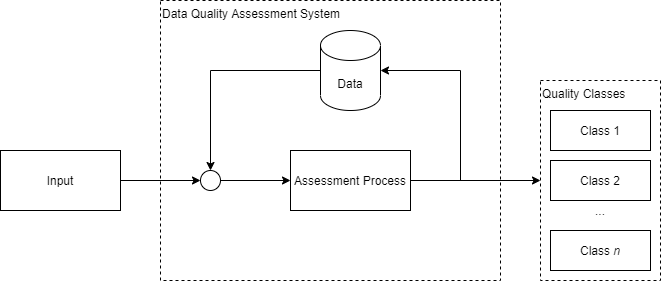
\includegraphics[width=0.9\textwidth]{figures/dq-system.png}
%     \caption{}
%     \label{fig:dq-system}
% \end{figure}
% \FloatBarrier

% \subsection{System Stability}

% In principle, we can classify three types of system stability:

% \begin{enumerate}
%     \item Stable System (Absolute and Conditional stability);
%     \item Marginally Stable System;
%     \item Unstable System.
% \end{enumerate}

% \subsection{Analytics Types}

% \begin{itemize}
%     \item Descriptive – what happened in the past;
%     \item Diagnostic – why something happened in the past;
%     \item Predictive – what is most likely to happen in the future;
%     \item Prescriptive – recommends actions to affect those outcomes.
% \end{itemize}

% DQ dimensions vs DQ metrics

% "Confidetial/secret data will always have limited quality."
